\documentclass[conference]{IEEEtran}

\usepackage[utf8x]{inputenc}

\usepackage{dcolumn}
\usepackage{graphicx}
\usepackage{epsfig}
\usepackage{amssymb}
\usepackage{amsmath}
\usepackage{amsfonts}
\usepackage{subcaption}
\usepackage{multirow}
\usepackage{color}
\usepackage{array}
\usepackage{listings}
\lstset{language=C}

\usepackage{times}

\begin{document}

\title{Software-defined network support for transport resilience}

%\author{
%\alignauthor Jo\~{a}o Taveira Ara\'{u}jo\\
%        \email{j.araujo@ucl.ac.uk}
%\alignauthor Raul Landa \\
%        \email{r.landa@ucl.ac.uk}
%\alignauthor Kensuke Fukuda \\
%        \email{kensuke@nii.ac.jp}
%\alignauthor George Pavlou \\
%        \email{g.pavlou@ucl.ac.uk}
%\end{tabular}\newline\begin{tabular}{cc}
%    \affaddr{University College London} & \affaddr{University College London}\\
%    \affaddr{London, UK} & \affaddr{London, UK}\\
%}


% author names and affiliations
% use a multiple column layout for up to three different
% affiliations
\author{\IEEEauthorblockN{Jo\~{a}o Taveira Ara\'{u}jo, Ra\'{u}l Landa, Richard G. Clegg, George Pavlou}
\IEEEauthorblockA{University College London\\
Email: \{j.araujo, r.landa, r.clegg, g.pavlou\}@ucl.ac.uk}}
%\and
%\IEEEauthorblockN{Kensuke Fukuda}
%\IEEEauthorblockA{National Institute of Informatics\\
%kensuke@nii.ac.jp}}

\maketitle

\maketitle
\begin{abstract}
Existing methods for traffic resilience at the network and transport layers typically work in isolation, often resorting to inference in fault detection and recovery respectively.
This both duplicates functionality across layers, eroding efficiency, and leads to protracted recovery cycles, affecting responsiveness.
Such misalignment is particularly at odds with the unprecedented concentration of traffic in data-centers, in which network and hosts are managed in unison.

This paper advocates instead a cross-layer approach to traffic resilience.
The proposed architecture, INFLEX, builds on the abstractions provided by software-defined networking (SDN) to maintain multiple virtual forwarding planes which the network assigns to flows.
In case of path failure, transport protocols pro-actively request to switch plane in a manner which is unilaterally deployable by an edge domain, providing scalable end-to-end forwarding path resilience.


\end{abstract}

While the Internet has become evermore interconnected, exploring path diversity has been relegated to an afterthought in an architecture modeled around assumptions that no longer stand. 
Single-path forwarding as a paradigm arose not as a guiding principle, but as a natural aversion towards increasing both the complexity and cost of a resource starved network.
%engineering for scarcity worked, but cracking
Engineering for scarcity has propelled the Internet to an unprecedented scale, but problems arise when what was otherwise scarce becomes plentiful. 
Protocols designed to be bit conservative at the expense of latency have become technological anachronisms as bandwidth costs continue to plummet. 
Similarly, the notion of a router as a device merely capable of forwarding packets has long been obsolete as Moore's law continues to pave the way for greater functionality within the network. 
\ac{NAT}, \ac{DPI} or \ac{PEP} are all examples that when it comes to drawing a boundary between network and transport, the line begins to blur \cite{Ford:2008p34}.

%% paralelism increasing
Furthermore, parallelism seems to be a dominant trend at every level of the Internet architecture as a cost-effective means of increasing both performance and robustness. 
At the inter-domain level, the \ac{AS} graph is becoming flatter and more highly interconnected \cite{Haddadi:2010p129}. 
Within domains, the sheer complexity of managing paths has led to the streamlined design and deployment of \ac{MPLS} \cite{Rosen:2001p147}, implementing a fully fledged layer in its own right. 
At the edges the rise in multi-homing continues to increase the strain on an already overloaded routing architecture. 
Even within network components, parallelism is such that packet re-ordering can no longer be considered pathological \cite{Bennett:1999p120}.

Given these trends, one would expect the ability to pool traffic across such emergent path diversity to have become a network primitive. 
In reality, each stakeholder in the Internet architecture seems to balance traffic according to their needs while attempting to remain inconspicuous to others. 
At best, this interaction between stakeholders can be seen as a form of commensalism, where one entity can extract benefits while others remain unaffected. 
At worse, the competitive nature of the tussle \cite{Clark:2005p67} that ensues can spiral into a situation where few profit.

This chapter investigates the nature of this antagonism between network and endpoints and reflects on how the Internet can accommodate the needs of both through the use of \ac{PREFLEX}, a proposed architecture for balancing congestion which foments mutualism between end-hosts and edge network providers.

\section{Openflow background}
\label{section:inflex:background}

%layout
Software defined networks decouple the data plane and control plane, allowing both to evolve independently.
A traditional instantiation of a software defined network for data centres is shown in figure \ref{fig:ofparch}.
Each physical host runs a number of virtual machines, each connected locally through a edge, software-based switch (such as OpenVSwitch \cite{openvswitch}) running on the underlying physical host operating system, which will be denoted as \emph{dom0}.
This switch is in turn connected to further forwarding devices, ensuring access to a wider network.
The forwarding logic of each device can be accessed and configured by a controller through the establishment of a control channel through a common protocol, of which Openflow is the most widely used \cite{McKeown:2008:OEI:1355734.1355746}.
Both software and physical switches are indistinguishable from a controller's perspective: \emph{how} a device implements Openflow is immaterial, so long as a forwarding device conforms to the given \ac{API}.

\begin{figure}
    \centering
    \begin{subfigure}[b]{0.5\linewidth}
    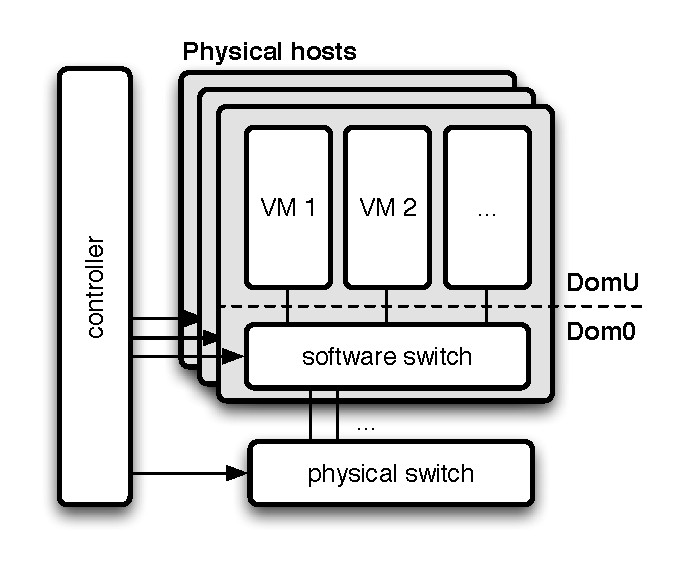
\includegraphics[width=0.9\linewidth]{figures/inflex/ofparch}
    \caption{\label{fig:ofparch}}
    \end{subfigure}%
    \begin{subfigure}[b]{0.5\linewidth}
    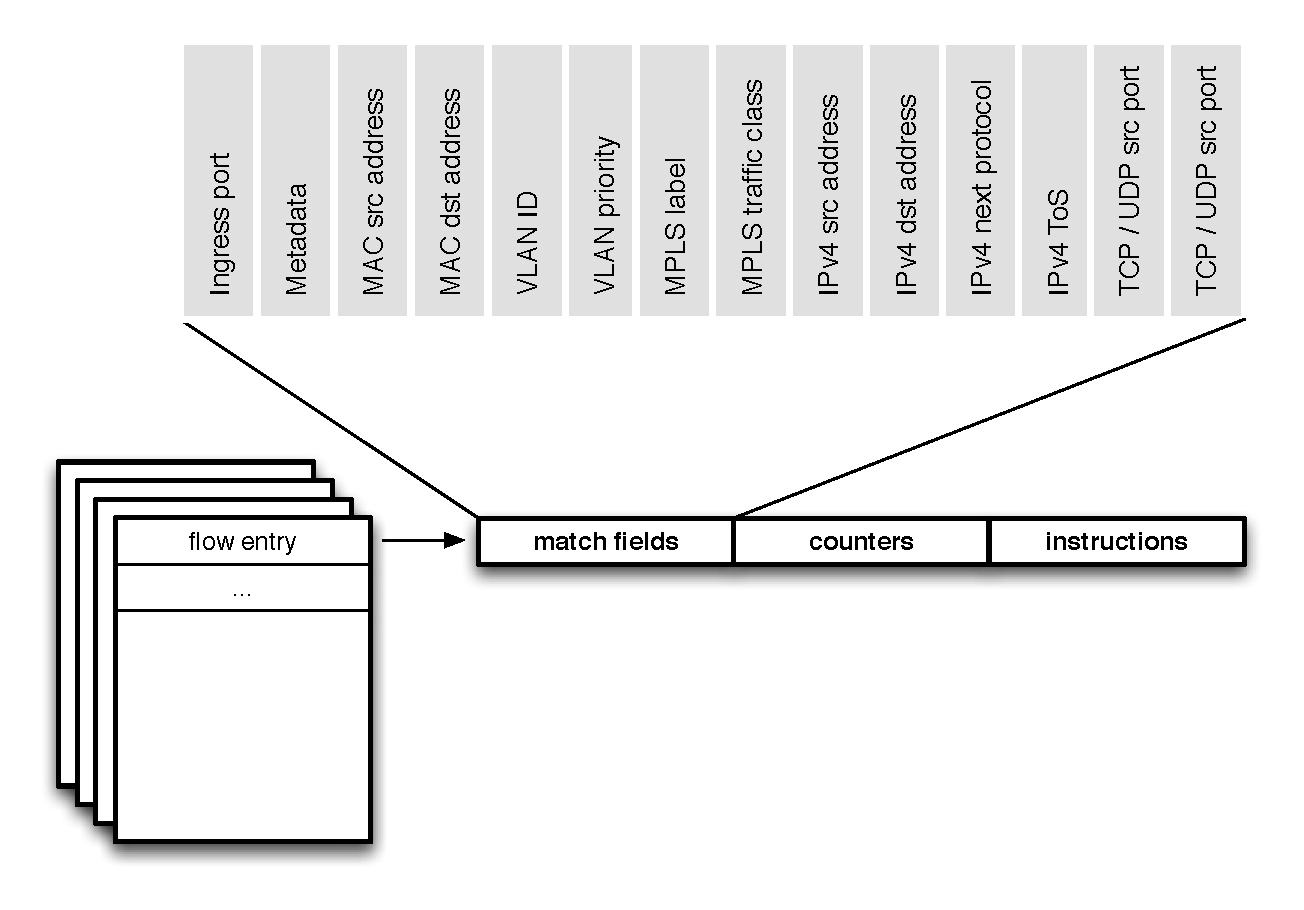
\includegraphics[width=0.9\linewidth]{figures/inflex/ofptable}
    \caption{\label{fig:ofptable}}
    \end{subfigure}
    \caption{Openflow (\subref{fig:ofparch}) architecture and (\subref{fig:ofptable}) flow entry structure.}
\end{figure}

% flow table / entry
An Openflow flow table is composed of multiple flow entries, shown in figure \ref{fig:ofptable}.
Each flow entry is comprised of a pattern to be matched, and the corresponding \emph{instructions} to be executed. 
The \emph{match fields} over which an entry can be compared span from data link to transport layers, covering not only source and destination addresses at each protocol header, but also traffic classes and labels for \ac{VLAN}, \ac{MPLS} and \ac{IPv4} headers.
% instructions?
Additionally, a \emph{counter} keeps track of the number of times the entry is matched.
If more than one matching entry is found, only the entry with the highest \emph{priority} is processed.
Finally, each entry has a pair of associated \emph{timeout} values: a soft timeout, within which an entry is expired if no matching packet arrives, and a hard timeout, by which an entry is irrevocably expired.
If neither timeout is set, a flow entry persists indefinitely.

% processing pipeline
An Openflow switch in turn maintains multiple flow tables.
Every packet received at an Openflow compliant switch is processed along a pipeline which starts by matching the packet against \emph{table 0}.
From this first, default table, corresponding \emph{instructions} may redirect the packet for further matching against another table, thereby chaining processing.
This pipeline processing ceases once a matching entry fails to include a redirection request, with the accumulated instruction set being executed.
In addition to redirections, valid instructions include modifying packet fields, pushing and popping packet tags, and defining through which ports a packet should be forwarded.
%instructions?
If at any point no matching entry is found, the packet is buffered at the switch, and the truncated packet header is sent to the controller.
% controller
Based on the header contents, a controller may decide to install a new flow entry on the switch, or allow the packet to be dropped altogether.
Compared to the underlying, abstracted network elements which compose the data path, the controller is often expected to be entirely software based, and as such is not constrained in how it should process packets.
In practice, this freedom is curbed as increasing complexity at the controller both reduces the rate at which packets are processed, as well as increasing latency for packets buffered at the switch.

% 2 tradeoffs: 
The overall performance of the described architecture is subject to two further critical trade-offs.
% - granularity vs speed
Firstly, the granularity at which flow entries are installed determines how often a controller is called to intervene.
While installing an entry at a flow granularity may allow fine-grained control of resources, it increases both the load on the controller and the latency of the withheld packet.
Conversely, as the granularity becomes coarser, the overhead incurred by the controller is reduced at the cost of flexibility in controlling traffic.
% - omniscience vs fault tolerance
Secondly, controller placement is critical \cite{Heller:2012:CPP:2342441.2342444}.
At one extreme, a fully centralized controller is omniscient within a domain at the expense of reliability and scalability.
At the other, a distributed system of controllers forsakes consistency and liveness in order to scale robustly.

\section{Design considerations}
\label{section:design}

%\subsection{Multipath state}
%\subsection{Network granularity}
%\subsection{Deployment}
%\subsection{Flowlet?}

\ac{SDN} provides an abstraction over which different architectural paradigms can be adapted and even coexist.
It does not however prescribe or advocate a specific design -- network practitioners must still consider system properties when grappling with fundamental tradeoffs affecting consistency, isolation, reliability and efficiency.
This section provides design considerations for scalable traffic management based on observations obtained from the data collected in chapters \ref{chapter:malawi} and \ref{chapter:rate}.

\begin{figure}[t]
    \centering
    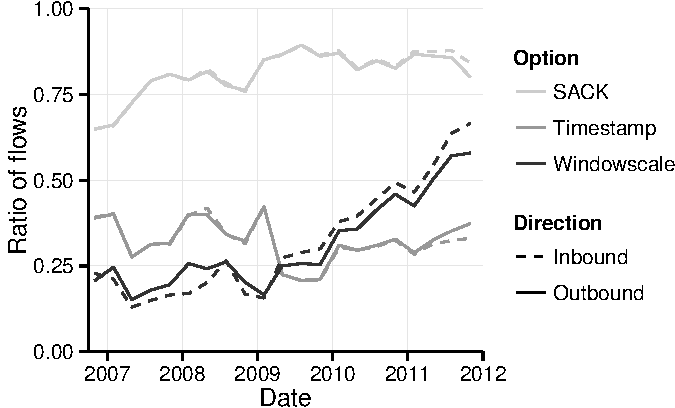
\includegraphics[width=4.0in]{figures/inflex/options}
    \caption{\acs{TCP} option usage \label{fig:wscale}}
    \hfill
\end{figure}

Ideally resilience could be implemented at the transport layer alone, for the same motives rate control is best left to end-hosts: ultimately, the host is best positioned to detect end-to-end path faults and can often react over shorter timescales than the network, which must concern itself with reconvergence.
This approach for path fail-over was a significant feature in \ac{SCTP} \cite{rfc4960}.
Unfortunately, deployment of \ac{SCTP} has been negligible in over a decade since standardization, in part because the pervasiveness of middleboxes has significantly affected the ability for new transport protocols to be deployed.
More recently \ac{MPTCP} \cite{Wischik:2008p137} has been proposed addressing many of the same concerns as \ac{SCTP} whilst maintaining the same wire format as \ac{TCP}, thereby ensuring middlebox compatibility.
Despite this, widespread deployment is far from guaranteed, and is largely tied to the rate of \ac{OS} adoption.
As a reference point, figure \ref{fig:wscale} tracks the use of three \ac{TCP} options by overall volume in flows across both directions in the \ac{MAWI} dataset.
While \ac{SACK} is successfully negotiated for most connections, the deployment of the timestamp and windowscale options has lagged.
While the former primarily assists in provide more accurate \ac{RTT} estimates, the latter is critical for performance: without windowscale negotiation, a sender's congestion window cannot exceed 65KB.
Despite offering a clear benefit to both endpoints, being simple to implement and incurring a low overhead, windowscale deployment has only recently picked up momentum, two decades since standardization.
Expecting substantial deployment of a more complex and costly extension such as \ac{MPTCP} over the near future is likely optimistic.
Critically, transport extensions require receiver adoption and are therefore subject to the willingness and ability of users to upgrade their OS.

{\COMMENT missing: PREFLEX problems here. Concept of deployability changed.}

\textbf{Receiver side deployment of even modest \ac{TCP} extensions can be protracted, even when incentives are aligned}. 
Rather than proposing a path for incremental deployment, this work focuses on how to obtain similar benefits immediately -- modifying sender side hosts only. 
A host, however, cannot directly affect routing without changing destination address, which would break legacy \ac{TCP} receiver side implementations. Additional extensions are required on the sender side network to enable multipath forwarding.
Conventional wisdom suggests that maintaining parallel routing planes requires a proportional increase in table size \cite{NingWang:2008p145}, which itself can be subject to exponential growth.
In practice however, this state can be significantly reduced by forsaking coverage for a small proportion of traffic.
Rather than reflect the entirety of its potential path diversity for all traffic, an edge provider can instead provide additional routing planes for only a subset of popular prefixes.

\begin{figure}[t]
    \begin{subfigure}[b]{0.5\linewidth}
        \centering
        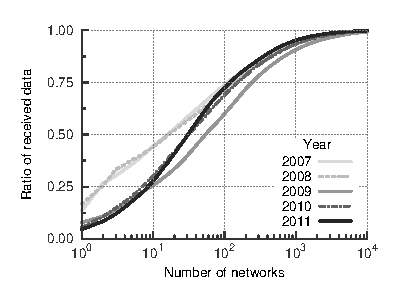
\includegraphics[width=3.0in]{figures/inflex/ecdf_network_dst_data_bytes_from_10000.eps}
        \caption{\label{prefix_in}}
    \end{subfigure}
    \begin{subfigure}[b]{0.5\linewidth}
        \centering
        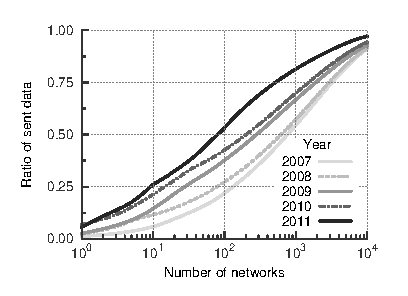
\includegraphics[width=3.0in]{figures/inflex/ecdf_network_dst_data_bytes_to_10000.eps}
        \caption{\label{prefix_out}}
    \end{subfigure}%
    \caption{\acs{CDF} of traffic by announced network prefix for (\subref{prefix_in}) inbound and (\subref{prefix_out}) outbound traffic.\label{fig:prefix}}
    \hfill
\end{figure}

The extent to which such a gain is possible for the \ac{MAWI} dataset is quantified in figure \ref{fig:prefix}, which displays the cumulative distribution function of outbound traffic across network prefixes announced by BGP neighbours.
Over five years, traffic to approximately 340,000 unique prefixes was observed.
Invariably however, an increasing amount is sent to a small group of prefixes -- by 2011, over 50\% of traffic went to the top 100 prefixes alone.
This reflects ongoing structural changes in the Internet architecture as content providers interconnect directly edge, \emph{eyeball} networks, and content becomes increasingly consolidated across a set of large content providers and national and regional ISPs.

\textbf{Multipath routing state can be significantly reduced by covering fewer destinations while still benefiting most traffic}. 
Within the \ac{MAWI} dataset virtually all inbound and outbound traffic could be mapped to 10,000 unique network prefixes. 
Existing \ac{SDN} tools such as RouteFlow \cite{Rothenberg:2012:RRC:2342441.2342445} are already capable of overlaying routing on commodity switches, but the incurred overhead can still be a concern for production networks.
Rather than address the scalability challenges inherent to multipath routing directly, these results suggest that a tangible deployment path lies instead in reducing the scope over which it is applied.


\section{Architecture}
\label{section:inflex:arch}

This section describes INFLEX, an architecture which provides edge domains with greater end-to-end resilience.
Rather than probing paths through active or passive means, the network delegates the responsibility for fault detection to end-hosts.
The system relies on packet marking at the host to select a path through the local domain.
This provides far greater scalability in terms of the proportion of traffic and destinations which can be covered, at the cost of requiring small changes to the end-host \ac{TCP}/\ac{IP} stack.
INFLEX is therefore particularly suited for managed environments, such as datacenters or enterprise networks, which not only have greater control over the end-host operating system, but also generate large volumes of traffic towards destinations which cannot be readily upgraded.

An overview of the proposed architecture as applied to a single domain is shown in figure \ref{fig:inflexarch}.
Hosts are connected to the local network through an Openflow-enabled \emph{edge switch}.
While edge switches typically reside within each physical machine, alternative aggregation levels such as the top of rack or end of row may also be used.
Each switch is configured by a specialized controller which resides locally, referred to as an \emph{inflector}.
The local network is configured by a centralized routing controller to provide multiple \emph{virtual routing planes}.
While these planes are necessarily intradomain in scope, some degree of interdomain diversity can also be achieved by changing egress node.

The core of the architecture relies on repurposing the \ac{DS} field in each \ac{IP} packet to provide an in-band signalling channel between the end-host and the inflector.
The header on inbound traffic is set by the edge switch and read by the host, and is used by the inflector to signal which plane a flow has been assigned to.
The header on outbound traffic is set by the host and read by the edge switch, and is used by the transport protocol to ensure that all traffic for the flow is forwarded along the given plane.
Hosts can request a new plane to be assigned by the inflector in case of an end-to-end path fault; this provides efficient cross-layer failure recovery.
The \ac{DS} standard \cite{Blake:1998p370} reserves a pool of code points for local use identified by setting the right-most bit, henceforth referred to as the INFLEX $flag$.
When set, the rest of the \ac{DS} field should be interpreted as containing two fields, shown in figure \ref{fig:inflexarch}. 
An \ac{INF} $label$, which determines the plane over which a packet is forwarded, and an $echo$ bit, which explicitly signals a request from the host or a reply from the network.
The remainder of the description of INFLEX is split across its main components: the end-hosts, the edge switch and the inflector.

\begin{figure}
    \begin{subfigure}[b]{1.0\linewidth}
    \centering
    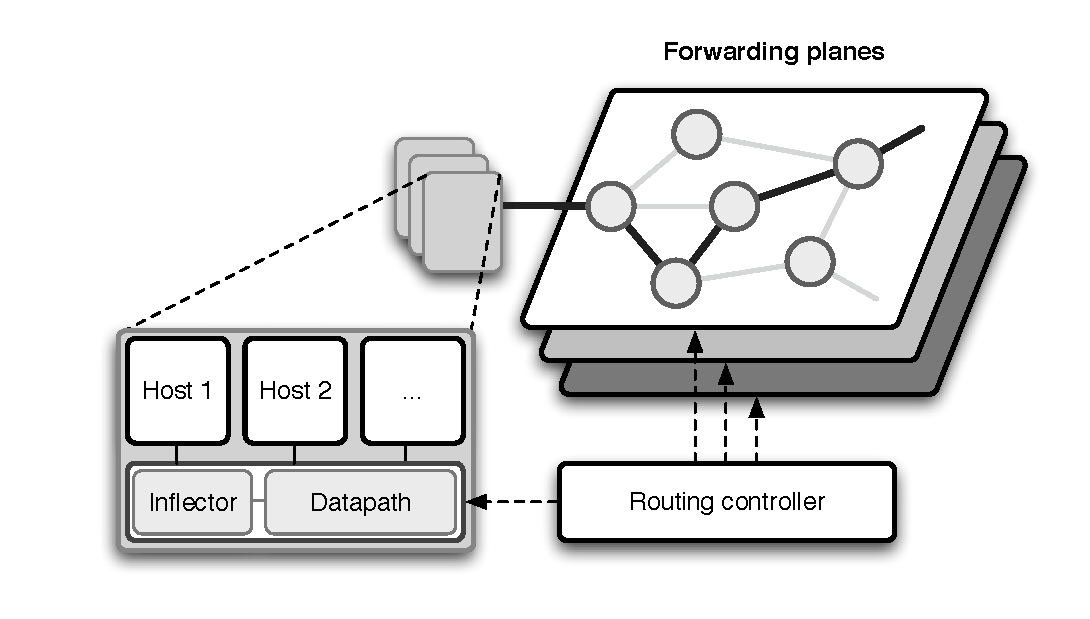
\includegraphics[width=0.7\linewidth]{figures/inflex/arch}
    %\caption{\label{fig:inflexarch}}
    \end{subfigure}
    \begin{subfigure}[b]{1.0\linewidth}
    \centering
    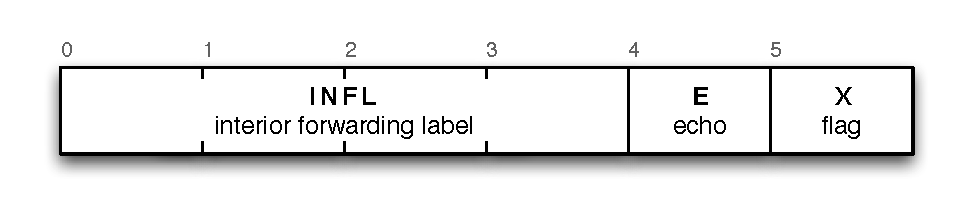
\includegraphics[width=0.5\linewidth]{figures/inflex/header}
    %\caption{\label{fig:inflexheader}}
    \end{subfigure}
    \caption[INFLEX architecture and header.]{INFLEX architecture (above) and header (below). The edge switch forwards traffic across virtual planes set up by a centralized routing service.
    \label{fig:inflexarch}}
\end{figure}

\subsection{INFLEX end-hosts}
\label{section:inflex:host}

INFLEX hosts set the \ac{INF} label of outbound packets according to the value assigned by the inflector, reproducing the path re-feedback design pattern introduced in chapter \ref{chapter:preflex}.
INFLEX however cannot rely on marking by the remote endpoint to trigger network action, as this has been shown to be essentially undeployable.
Instead, path requests are initiated by the sender, which must then await for a network reply piggybacked on a returning packet.

The changes required to support this at the sender side network stack are minimal, and are illustrated in figure \ref{fig:stack}.
Every transport connection occurs over a socket, a local structure containing the variables associated to the ongoing flow.
At the network layer, the local socket has a \ac{DS} value which is copied to every outbound packet (point 1).
Within INFLEX, the transport protocol can trigger a request (point 2), which leads to a network response contained in incoming packets (point 3).

Assume a transport protocol wishes to switch the plane it is currently assigned.
With INFLEX, it can send an \emph{inflection request} by setting the $echo$ bit of the local \ac{DS} field (point 2, figure \ref{fig:stack}).
All subsequent outbound packets will be marked with the resulting value.
The network layer then proceeds to inspect inbound packets, waiting for a network response, as delineated in figure \ref{fig:tcpcode}.
After demuxing an incoming packet, $pkt$, to the corresponding socket, $sock$, a receiver first verifies whether the INFLEX flag is set on the incoming packet (line 2), establishing whether the underlying network supports INFLEX for the given connection.
The receiver must then decide whether it should change the virtual plane the socket is currently assigned.
This can only happen under two conditions.
Firstly, if the \ac{DS} value for the current socket does not have the INFLEX flag set (line 3).
This typically occurs on flow start, where a connection is spawned with a default \ac{DS} value.
Secondly, if the local \ac{DS} value has the echo bit set, there is a \emph{pending} inflection request.
If the incoming packet has the same bit set, it corresponds to the network \emph{reply} (line 4).
Under both previous cases, the connection switches forwarding plane by copy the interior forwarding label from the incoming packet to the local socket, and setting the INFLEX flag (lines 5-6).
These changes are all applied at the \ac{IP} layer -- transport protocols need only to decide when to send inflection requests -- while applications can remain unchanged.

\begin{figure}
    \begin{subfigure}[b]{0.4\linewidth}
        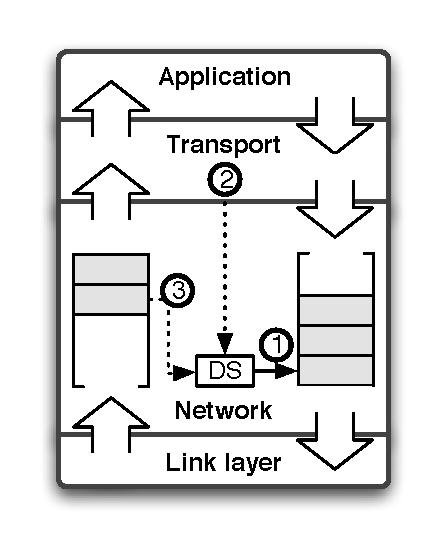
\includegraphics[width=0.9\linewidth]{figures/inflex/stack}
        \caption{\label{fig:stack}}
    \end{subfigure}%
    \begin{subfigure}[b]{0.6\linewidth}
        \vspace*{1.0in}
        \lstset{
        language=C,                % choose the language of the code
        basicstyle=\footnotesize\ttfamily,
        numbers=left,                   % where to put the line-numbers
        stepnumber=1,                   % the step between two line-numbers.
        numbersep=5pt,                  % how far the line-numbers are from the code
        %  backgroundcolor=\color{white},  % choose the background color. You must add \usepackage{color}
        showspaces=false,               % show spaces adding particular underscores
        numberstyle=\scriptsize,
        showstringspaces=false,         % underline spaces within strings
        showtabs=false,                 % show tabs within strings adding particular underscores
        tabsize=2,                      % sets default tabsize to 2 spaces
        captionpos=n,                   % sets the caption-position to bottom
        breaklines=true,                % sets automatic line breaking
        breakatwhitespace=true,         % sets if automatic breaks should only happen at whitespace
        title=\lstname,                 % show the filename of files included with \lstinputlisting;
        }
        \lstinputlisting{\locfolder/tcpapi.c}
        \caption{\label{fig:tcpcode}}
    \end{subfigure}
    \caption[INFLEX host modifications.]{INFLEX (\subref{fig:stack}) host stack and (\subref{fig:tcpcode}) pseudo-code for packet reception.}
\end{figure}

% inflection request
\subsection{The edge switch}

% what is it
The edge switch is primarily responsible for mapping INFLEX marked packets to the appropriate forwarding plane.
On start up its datapath is configured by the local \emph{inflector}, which installs the appropriate flow entries on it in order to construct the processing pipeline in figure \ref{fig:pipeline}.
This pipeline can be partitioned into three distinct blocks, responsible for \emph{triaging}, \emph{policing} and \emph{inflecting} packets.
For clarity, the processing pipeline is conceptually described as a sequence of flow matches across distinct tables.
In practice, an implementer is free to collapse flow tables and entries to improve performance.
An important safeguard is that a legacy pipeline must be present, establishing a default forwarding plane expected to be used by traffic to which INFLEX is not applicable.

\begin{figure}
    \centering
    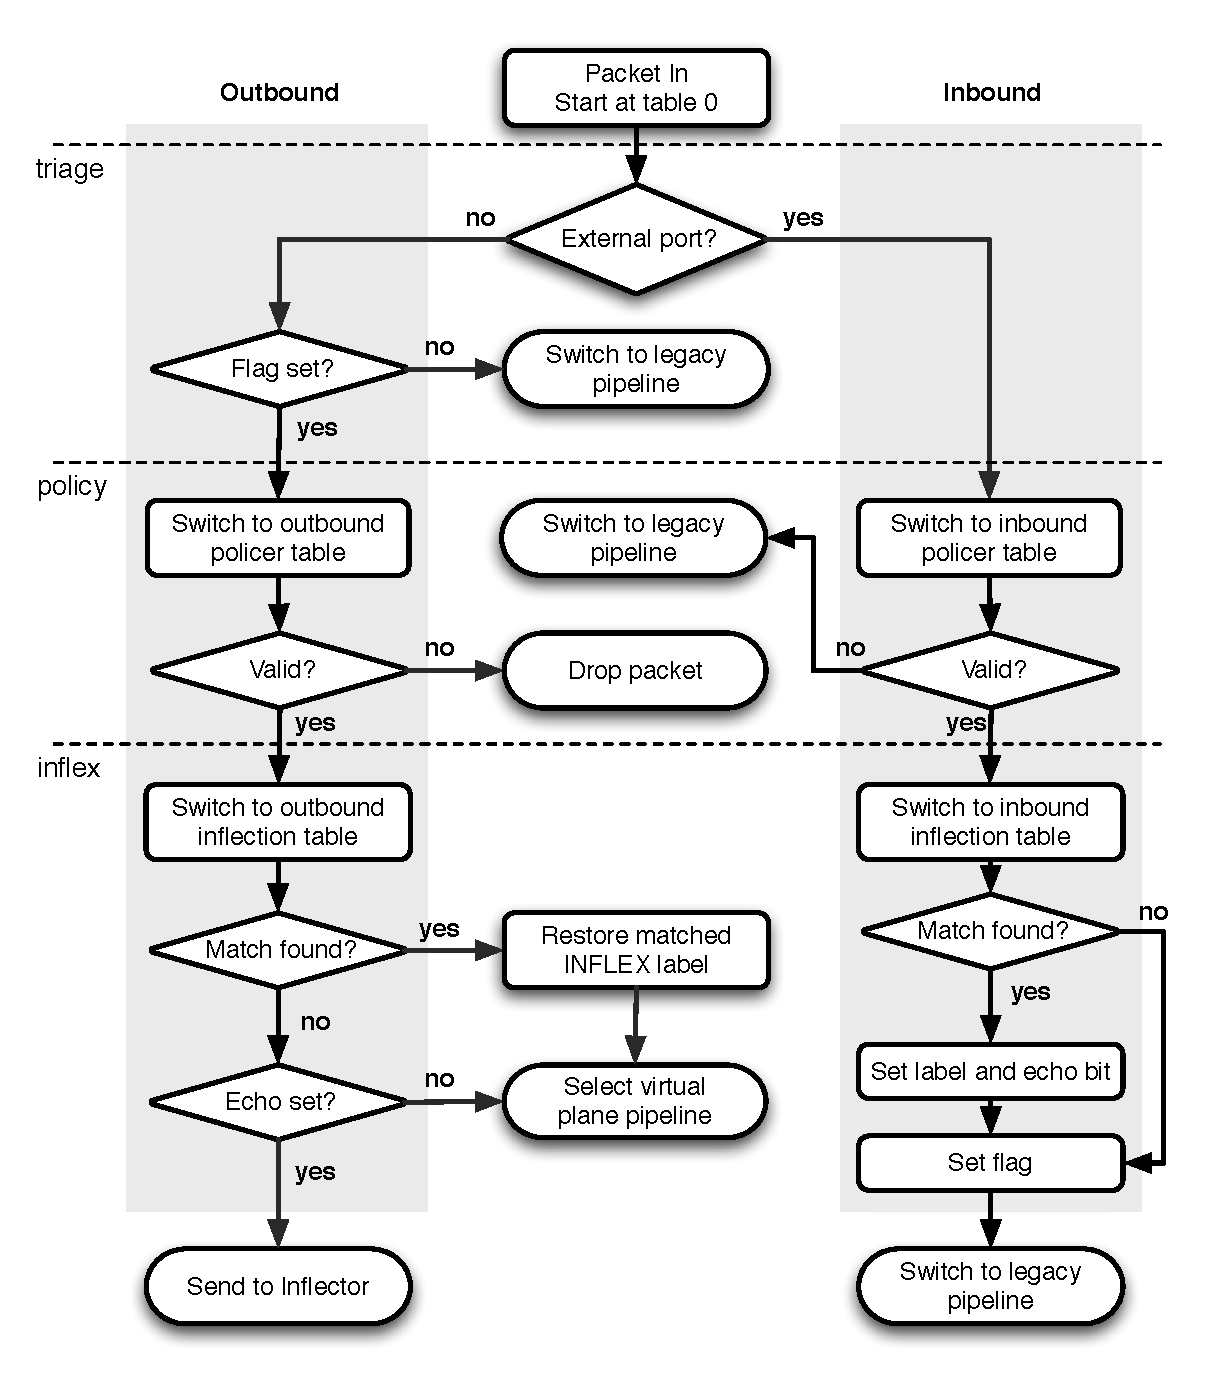
\includegraphics[width=3.5in]{figures/inflex/flowchart}
    \caption{Pipeline installed to the edge switch datapath.}
    \label{fig:pipeline}
\end{figure}

The \emph{triage} phase is responsible for distinguishing whether a packet is \emph{capable} of using INFLEX.
Firstly, INFLEX is only applicable to \ac{IP} packets.
Traffic is then differentiated according to the port on which the packet arrived: if connected to a host, the interface is said to be \emph{internal}, otherwise it is \emph{external}.
Any inbound \ac{IP} traffic may potentially be INFLEX capable and as such can proceed to the next stage.
For outbound \ac{IP} traffic, only packets with the INFLEX flag set require further processing.
Packets for which this flag is not set are assumed to be legacy traffic.

The \emph{policy} phase decides whether a packet is \emph{permitted} to use INFLEX.
For either direction, a packet is compared against a policer table, which contains a set of rules describing local policy concerning INFLEX usage.
The rules applied to each direction however may differ, particularly since outbound packets can be further scrutinized according to the INF $label$.
For example, this allows the outbound policer to enforce which virtual planes are available to specific tenants or applications.
For this reason, the action applied if a packet is matched within the policer table also differs according to direction.
For inbound traffic, a matching rule indicates that the packet does not satisfy local requirements for INFLEX use, and is consequently treated as legacy traffic.
For outbound traffic, a packet is already marked as being INFLEX capable.
Any matching entry therefore indicates that it is in violation of local policy and should consequently be dropped.

Finally, the \emph{inflex} phase processes the respective header and forwards the packet.
A packet is first matched against an \emph{inflection} table in either direction.
This table is detailed in the next section, and can be assumed to contain no matching entry initially.
For outbound traffic, the packet is typically redirected to the  plane mapped by the interior forwarding label.
The one exception are inflection requests, which are forwarded to the local inflector for further processing.
For inbound traffic, the INFLEX flag is marked in order to notify hosts that the flow is INFLEX capable, and the packet is then processed according to the legacy pipeline.

\subsection{The inflector}

% XXX
Each edge switch is controlled by an inflector, an \ac{SDN} controller expected to reside locally.
An inflector is firstly responsible for configuring the underlying datapath according to the previously described pipeline.
Secondly, an inflector must process inflection requests.

Inflection requests require network intervention in assigning a packet to a forwarding plane.
The dynamic nature of this decision process cannot readily be instantiated as a set of static rules at the edge switch, since a same flow must be able to be reassigned to a different plane in case of path faults.
Therefore, inflection requests intercepted at the edge switch must be sent to a controller for further processing.
Rather than overloading a centralized controller however, this decision can be taken locally -- since the inflector manages the local rules associated to each virtual network, it already has full knowledge of the routing table associated to each plane.
Upon receiving such a request, the inflector proceeds in three steps.
It first verifies which virtual networks maintain a valid route for the given destination address.
Given this list of potential planes, it then inspects local policy to verify which planes the packet is allowed to use.
The intercepted packet contains the plane which the flow is currently using -- this plane should be excluded from the candidate list unless there is no other option available.
Finally, a single plane, identified by an interior forwarding label, is selected from the resulting list of candidates.
The selection algorithm is not prescribed by the INFLEX specification, but a reasonable baseline is to select a routing entry proportionally to the assigned route weight.

Having selected an appropriate plane, the inflector installs forwarding rules into either \emph{inflection table}.
In the inbound direction, all packets matching the reverse flow are set to be marked with the corresponding \ac{INF} $label$.
This conveys the selected forwarding plane back to the host.
In the outbound direction, all packets matching the flow are to be processed according to the $label$.
This guarantees that any packet sent between the inflection request and its response are forwarded in a consistent manner.
Rules installed to the inflection tables are ephemeral by nature, with a hard timeout of 1 second (the minimum permitted in the Openflow standard).
This enables per-flow granularity with minimum flow state while also rate limiting inflection requests.
Furthermore, flow entries can be configured to be sent to the controller upon expiry.
This potentially allows the inflector to collect realtime information on the availability of each forwarding plane, allowing for further refinement of the plane selection algorithm.

\section{Performance Analysis}
%4.1) Balancing between two paths with high loss using fixed time unit
% using only loss-based balance in a simple regime where that works.
% Show how this converges quickly when one path suddenly gains
% background traffic (and hence loss).
%4.2) Balance between several paths with high loss and fixed time unit
% in simple regime where that works.
%4.3) Introduce experiment where equi-path is needed for probing and
% conservative is needed for low loss regime.
%4.4) Introduce experiment where time-scale tuning is needed to get
% good assessment of loss in low traffic regime.

This section evaluates \ac{PREFLEX} through simulation using ns-3 \cite{ns3}. 
Evaluating traditional traffic engineering methods typically involves abstracting traffic as flow aggregates, making large scale network performance analysis tractable.
\ac{PREFLEX} however balances traffic using loss rather than load, and focuses on improving end-user metrics as opposed to minimizing maximum link load.
As such, evaluating the proposed congestion balancer requires simulating end-to-end behaviour of traffic.

\subsection{Methodology}
\label{section:methodology}

Experimental validation is performed using the network topology displayed in figure \ref{fig:topo}. 
The topology links a client domain $C$ to a server domain $S$ through $N$ paths with equal bottlenecks $L_i$, and total bandwidth $B=\sum{L_i}$. 
While a domain is represented as a single entity in figure \ref{fig:topo}, each domain is composed by a traffic generator connected to a router. 
Client $C$ generates $G$ simultaneous \ac{HTTP}-like requests (or ``gets") from $S$ according to a specified distribution, described at the end of this section. 
As traffic flows from $S$ to $C$, the router within $S$ is responsible for balancing traffic over all available paths.

\begin{figure}
    \centering
    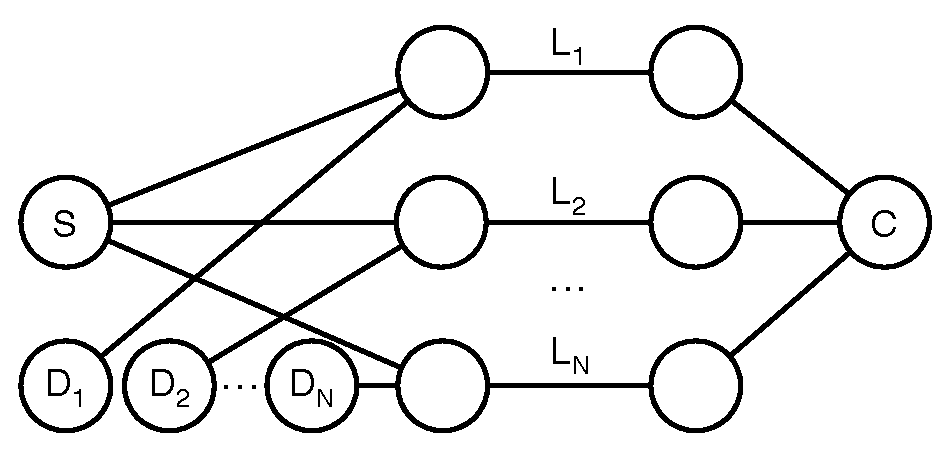
\includegraphics[width=2.5in]{figures/cate/topo}
    \caption{Simulation topology}
    \label{fig:topo}
\end{figure}

Across simulations, as the number of paths increases, total bandwidth $B$ and the number of simultaneous requests $G$ is fixed, providing insight into how efficiently \ac{PREFLEX} balances traffic as the granularity with which it can split traffic becomes coarser.

In order to evaluate how \ac{PREFLEX} shifts traffic in response to loss, additional ``dummy" servers $D_i$ are connected to $C$ through bottleneck link $L_i$.
The simulation runs for time $T$ and is partitioned into $N+2$ intervals starting on $s_i$, in which $s_0$ and $s_{N+1}$ have no traffic to $D_i$. 
Starting at time $s_i$, client $C$ generates $g_i$ requests to $D_i$ according to the same distribution as used to server $S$. 
All requests to $D_i$ end at time $s_{N+1}$. 
Equation \eqref{eq:si} sets the start time $s_i$ for requests to $D_i$ as a function of total simulation time $T$ and number of paths $N$. 
Likewise, equation \eqref{eq:gi} sets the number of simultaneous requests $g_i$ to $D_i$ as a function of $G$, the total number of requests to $S$, and $N$.
\begin{equation}
s_i = T\frac{i}{N+2}
\label{eq:si}
\end{equation}
\begin{equation}
\theta_i = \frac{\frac{1}{N+1-i}}{\sum{\frac{1}{N+1-i}}},  g_i = G\theta_i.
\label{eq:gi}
\end{equation}

Figure \ref{fig:demand} illustrates the number of simultaneous gets from $C$ to $D_i$ for $N=2$ (used in the example shown in figure \ref{fig:two}) and $N=4$. 
Generating cross-traffic in this manner serves two purposes. 
Firstly, $\sum{g_i}=G$, so independently of the number of concurrent paths, the maximum load in the system is $2G$. 
However, as the number of paths increases, the fluctuation in load for each path becomes smaller, stressing the sensitivity with which \ac{PREFLEX} must balance traffic. 
Secondly, the number of requests for each $D_i$ over time is the same. 
Over timescale $T$, equalisation appears to be an acceptable strategy but will however be shown to fail to make efficient use of available capacity. 
This is a fundamental limitation of offline traffic engineering, which is calculated over very long timescales and is unable to adapt as traffic routinely shifts.

\begin{figure}
    \begin{subfigure}[b]{.5\linewidth}
        \centering
        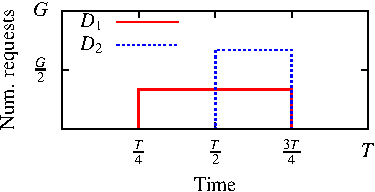
\includegraphics[width=2.25in]{figures/cate/dummy2-crop.pdf}
        \caption{$N=2$}\label{fig:1a}
    \end{subfigure}%
    \begin{subfigure}[b]{.5\linewidth}
        \centering
        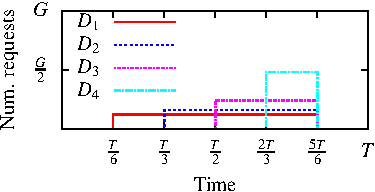
\includegraphics[width=2.25in]{figures/cate/dummy4-crop.pdf}
        \caption{$N=4$}\label{fig:1b}
    \end{subfigure}
    \caption[Number of requests to cross traffic servers.]{Number of requests from $C$ to cross traffic servers $D_i$ for different values of $N$}
    \label{fig:demand}
\end{figure}

The settings used for all simulations, including those previously shown in figure \ref{fig:two}, are as follows.
Total simulation time $T$ is set to $1200$ seconds, while total bandwidth $B$ is fixed at $240$Mbps. 
The number of requests $G$ sent from $C$ to $S$ is set to 240. 
Upon completing, a request is respawned after an idle period following an exponential distribution with a $15$s mean. 
Transfer size follows a Weibull distribution with an average value of $2$MB. 
While artificial, these values attempt to represent traffic to a single prefix with a file size that mimics the small but bursty nature of web traffic, which does not lend itself to being balanced by the end-host. 
\ac{PREFLEX} is configured with $\beta_E = 0.05$, $\mu_{min}=0.01/N$ and $\delta=0.005$.

\subsection{Varying bottleneck distribution}

For the remainder of this section, congestion balancing using \ac{PREFLEX} will be directly compared to equalisation, which mimics existing traffic engineering techniques based on hashing flow tuples for path assignment.
A useful reference point in interpreting results is to examine the case where all bottlenecks share the same bandwidth, $L_i=B/N$.
Under such conditions, figure \ref{fig:goodputeq} shows the goodput, calculated as the total data transfered to client $C$ by flows completed within $T$, as a proportion of total link bandwidth.
The bulk of goodput originates from server $S$, which is the only multi-homed domain.
If traffic is correctly balanced, servers $D_{1-N}$ should generate the same amount of goodput.
While both equalisation and congestion balancing saturate most available bandwidth, the former leads to disproportionate distribution of goodput amongst competing traffic. 
As loss is not equalised over all paths, the amount of goodput achieved by servers $D_i$ differs despite demand being similar.
\begin{figure}
    \centering
    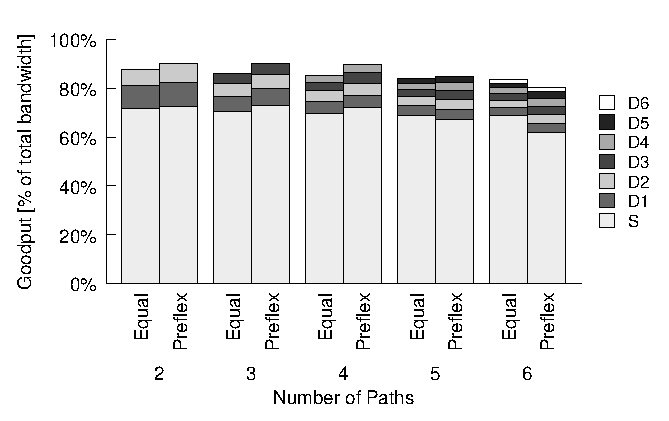
\includegraphics[width=4in]{figures/cate/eqbw}
    \caption[Goodput achieved over equal capacity links.]{Goodput relative to $B$ achieved by each server over equal capacity links.}
    \label{fig:goodputeq}
\end{figure}

In this scenario, equalisation can be seen as the optimal static TE solution, yet both approaches bear similar performance. 
With no knowledge of topology, link bandwidth or expected traffic matrices, \ac{PREFLEX} is able to adequately mimic the performance of the static TE solution for the case where such an approach is best suited.

\begin{figure}
    \centering
    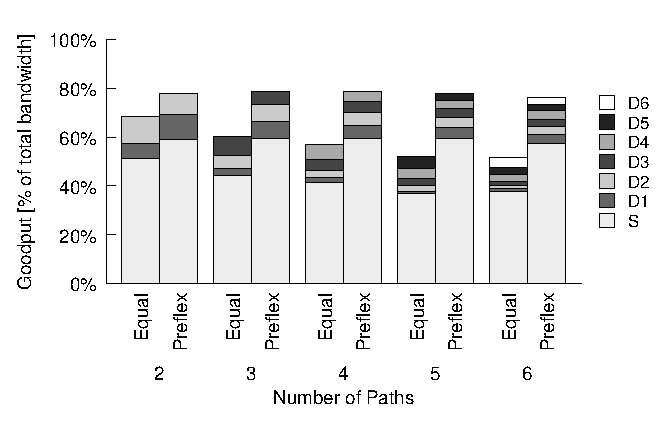
\includegraphics[width=4in]{figures/cate/diffbw}
    \caption[Goodput achieved over unequal capacity links.]{Goodput relative to $B$ achieved by each server over unequal capacity links.}
    \label{fig:goodputdiff}
\end{figure}

Where bottleneck bandwidth is unequal however equalisation is shown to be severely lacking.
The effect of differing bottlenecks is investigated by repeating previous simulations with the same total bandwidth $B$, but with $L_i$ set proportionally to $B$ in a similar manner to \eqref{eq:gi}, that is $L_i = \theta_i B$.
The ensuing results, shown in figure \ref{fig:goodputdiff}, highlight two significant shortcomings of equalisation which \ac{PREFLEX} overcomes. 
Firstly, goodput for $S$ drops as $N$ increases. 
Unable to realize it is overloading a path, equalisation is reduced to sending traffic over each link at approximately the same rate as the most congested link. 
In contrast, \ac{PREFLEX} detects congestion and adapts accordingly. 
Secondly, the incorrect distribution of traffic due to equalisation in $S$ distorts the goodput of competing traffic. 
While in \ac{PREFLEX} goodput from $D_{1-N}$ is perfectly balanced, with equalisation traffic crossing the most congested links are directly affected by another domain's inability to distribute traffic appropriately.
It may seem unfair to judge equalisation for cases where there is a mismatch in link capacity.
However, such a mismatch between link weight and path capacity arises regularly as operators adjust traffic engineering according to local conditions, with little thought spared for the impact this may have further downstream.

\begin{figure}
    \centering
    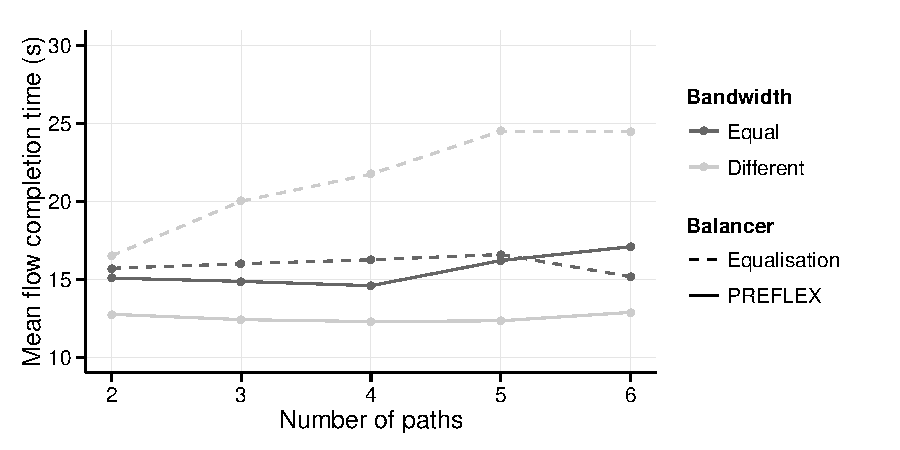
\includegraphics[width=3.2in]{figures/cate/duration}
    \caption[Mean flow completion time.]{Mean flow completion time for equal and differing bottleneck links.}
    \label{fig:duration}
\end{figure}

This impact is in turn perceived by users, who experience longer flow completion times, as shown in figure \ref{fig:duration}. 
In the equal bandwidth case the flow completion time is similar for both balancers.  
Where bandwidth differs however, balancing by congestion outperforms equalisation and maintains a stable performance even for all six paths.  
This shows that the algorithm scales well as the number of available paths increases. 

\section{Conclusions}
\label{section:conc}

This chapter presented INFLEX, a scalable and easily deployable end-to-end resilience framework based on the cross-layer control of an \ac{SDN}-enabled network layer.
The proposed architecture is shown to perform end-to-end path fail-over on much shorter time scales than existing solutions and is inherently modular, providing failure recovery through cooperation between end-hosts and the \ac{IP} network. 
In comparison to reliability mechanisms operating purely at the transport layer, such as \ac{MPTCP} or \ac{SCTP}, INFLEX enables transport resilience when communicating with legacy endpoints and does not require host multi-homing. 
Conversely, when compared to mechanisms operating purely at the network layer, INFLEX provides end-to-end visibility into path failures, allowing both fast detection and the implementation of remedial actions requiring fine-grained network control. 
The architecture  design presented is based on network measurements and implemented as a set of extensions to the Linux kernel and a popular Openflow controller. 
This implementation is then evaluated experimentally, demonstrating that high availability over multiple routing planes can be achieved without compromising network control scalability.



\bibliographystyle{IEEEtran}
{\footnotesize \bibliography{noms}}

\end{document}
